\section{Examples}
In this section, we show diverse examples to illustrate the usage of \name.
\begin{figure*}
    \includegraphics[width=\linewidth]{fig/ex5.eps}
    \caption{
        Illustrations of (a) the customized style, (b) the label plugin, (c) the lasso selection, (d) and (e) are two large-scale datasets.
%with 74,752 nodes 261,120 edges, and 35,590 nodes 572,915 edges
    }
    \label{fig:ex5}
\end{figure*}

\subsection{Basic Graph Drawing}
\autoref{fig:ex2} shows a basic case with three parts: initialization, loading data, and rendering. The `testData' illustrates the graph data format. In this example, the initialization part hangs the canvas to the document `main'.
\begin{figure}
    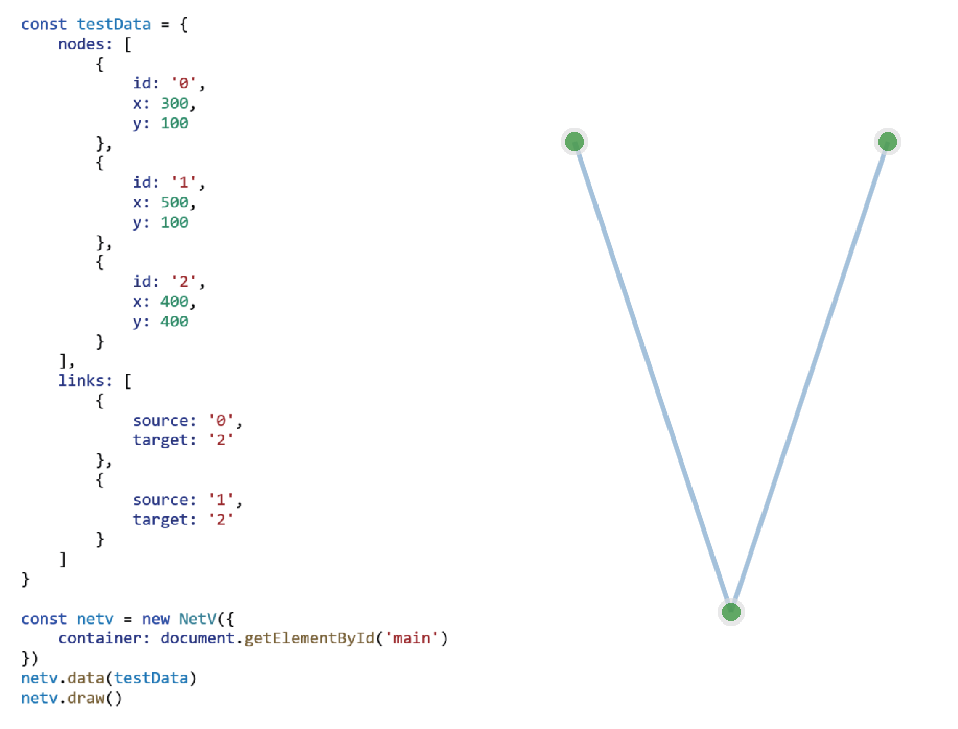
\includegraphics[width=\linewidth]{fig/ex2.eps}
    \caption{
        A basic unit of drawing three nodes and two edges.
    }
    \label{fig:ex2}
\end{figure}

\subsection{Customized Style}
The most important function of graph visualization is to draw a graph with different styles, such as color, stroke, radius, and position of elements.
\autoref{fig:ex5} shows the setting of customized styles by using \name. Developers can customize the style of each element and set the default style in the initialization part. In particular, initializzation configuration items are set in the `configs'.


% \begin{figure}
%     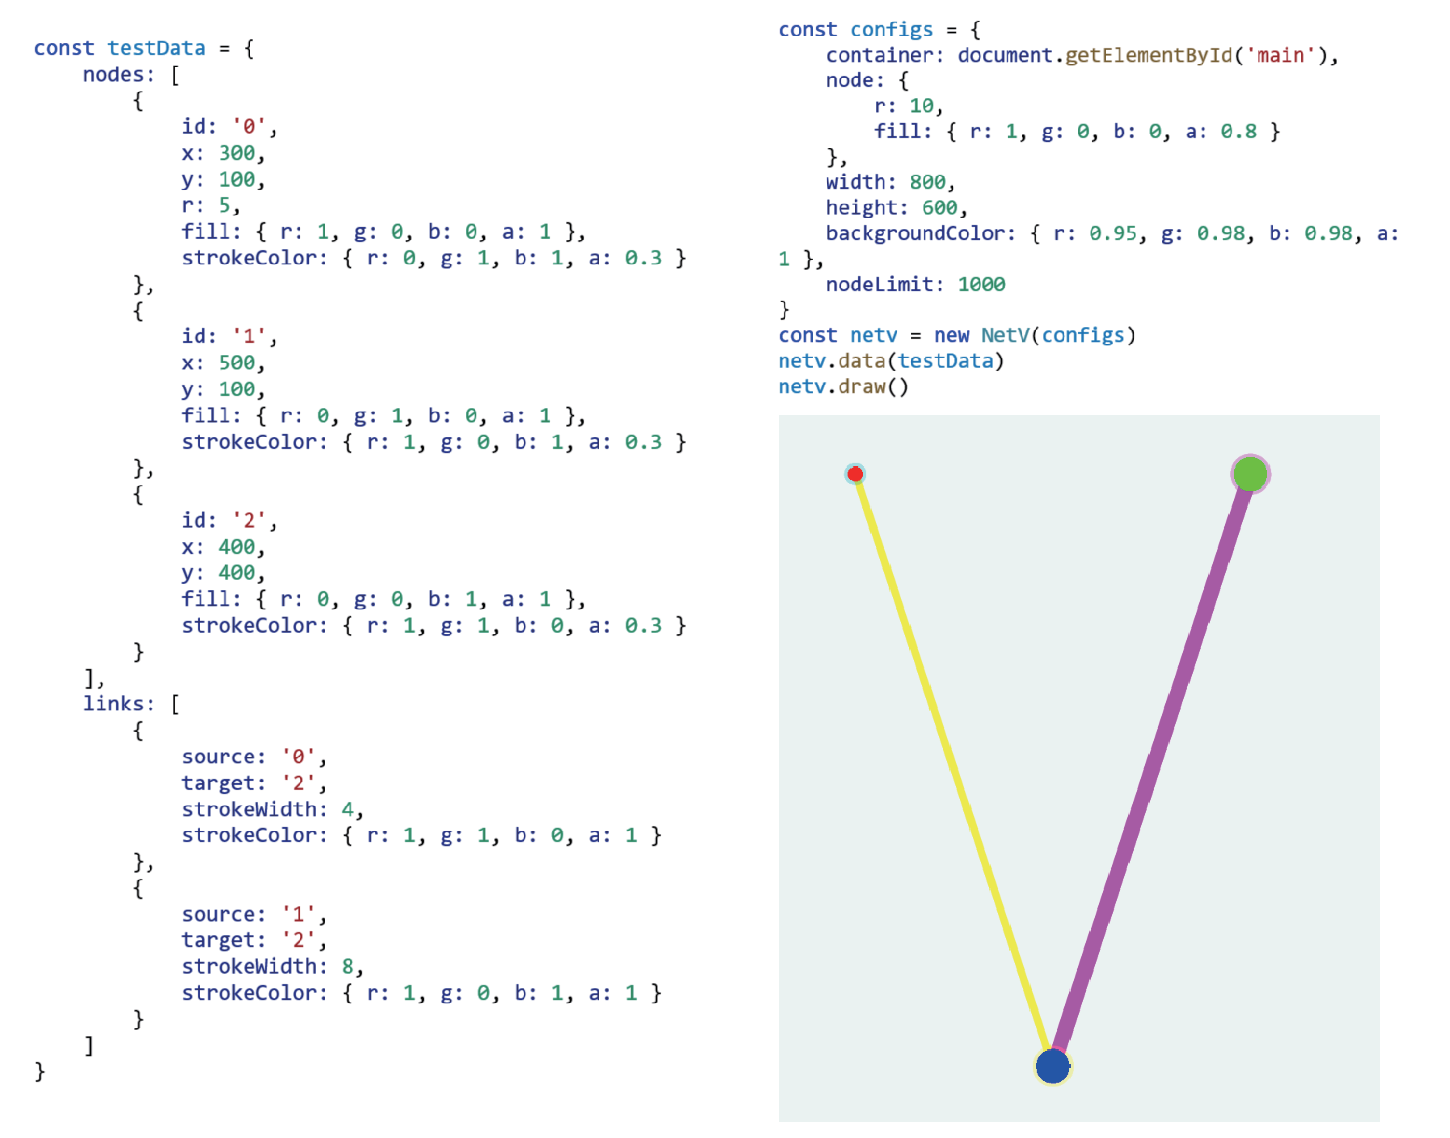
\includegraphics[width=\linewidth]{fig/ex1.eps}
%     \caption{
%         Customized style.
%     }
%     \label{fig:ex1}
% \end{figure}

% \subsection{Build-in datasets}
% \name supports build-in datasets for developers to construct a graph visualization (\autoref{fig:ex3}) quickly. The build-in datasets also support the attribute and the position of each node in the graph.
% developers can the radius and the color of nodes to encode different attributes of nodes.
% \begin{figure}
%     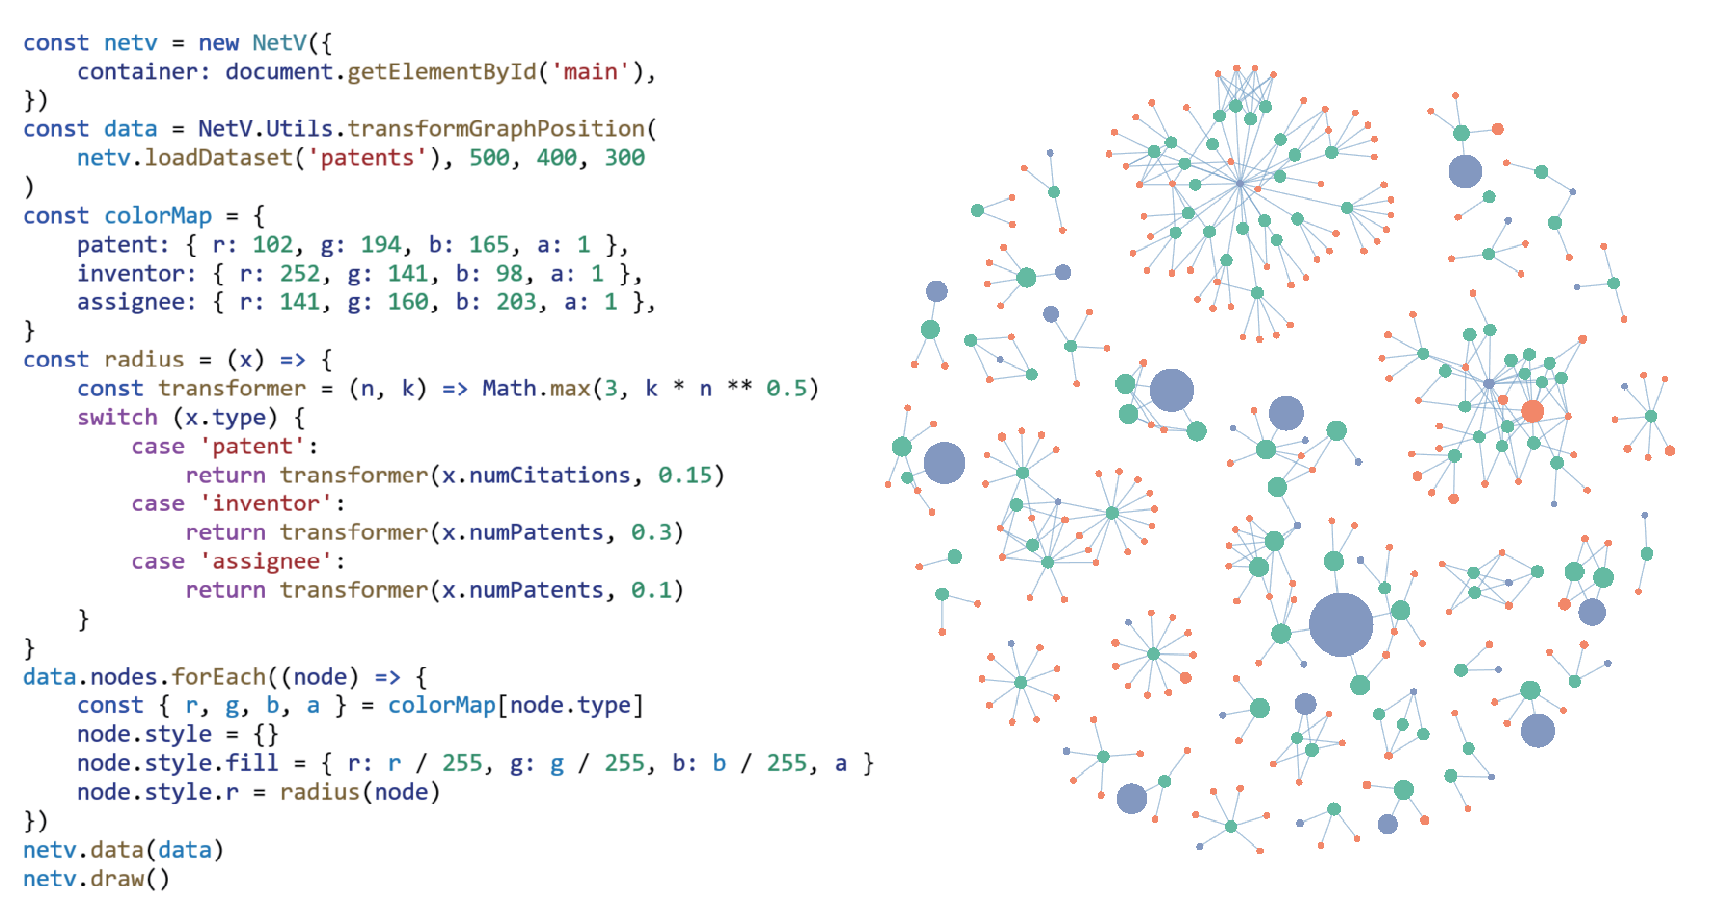
\includegraphics[width=\linewidth]{fig/ex3.eps}
%     \caption{
%         Build-in datasets.
%     }
%     \label{fig:ex3}
% \end{figure}

\subsection{Interaction}
A series of basic interactions are supported in \name, including pan, zoom, mousueover, and so no. \autoref{fig:ex8} (b) shows several build-in interactions.

\subsection{Plugin}

\name supports showing labels (\autoref{fig:ex5} (b)) with different drawing techniques such as SVG, Canvas, and WebGL. \name also supports lasso interaction (\autoref{fig:ex5} (c)) to select nodes and different layout algorithms. \autoref{fig:ex8} (a) shows plugin configurations of the label, lasso, and layout.


\begin{figure}
    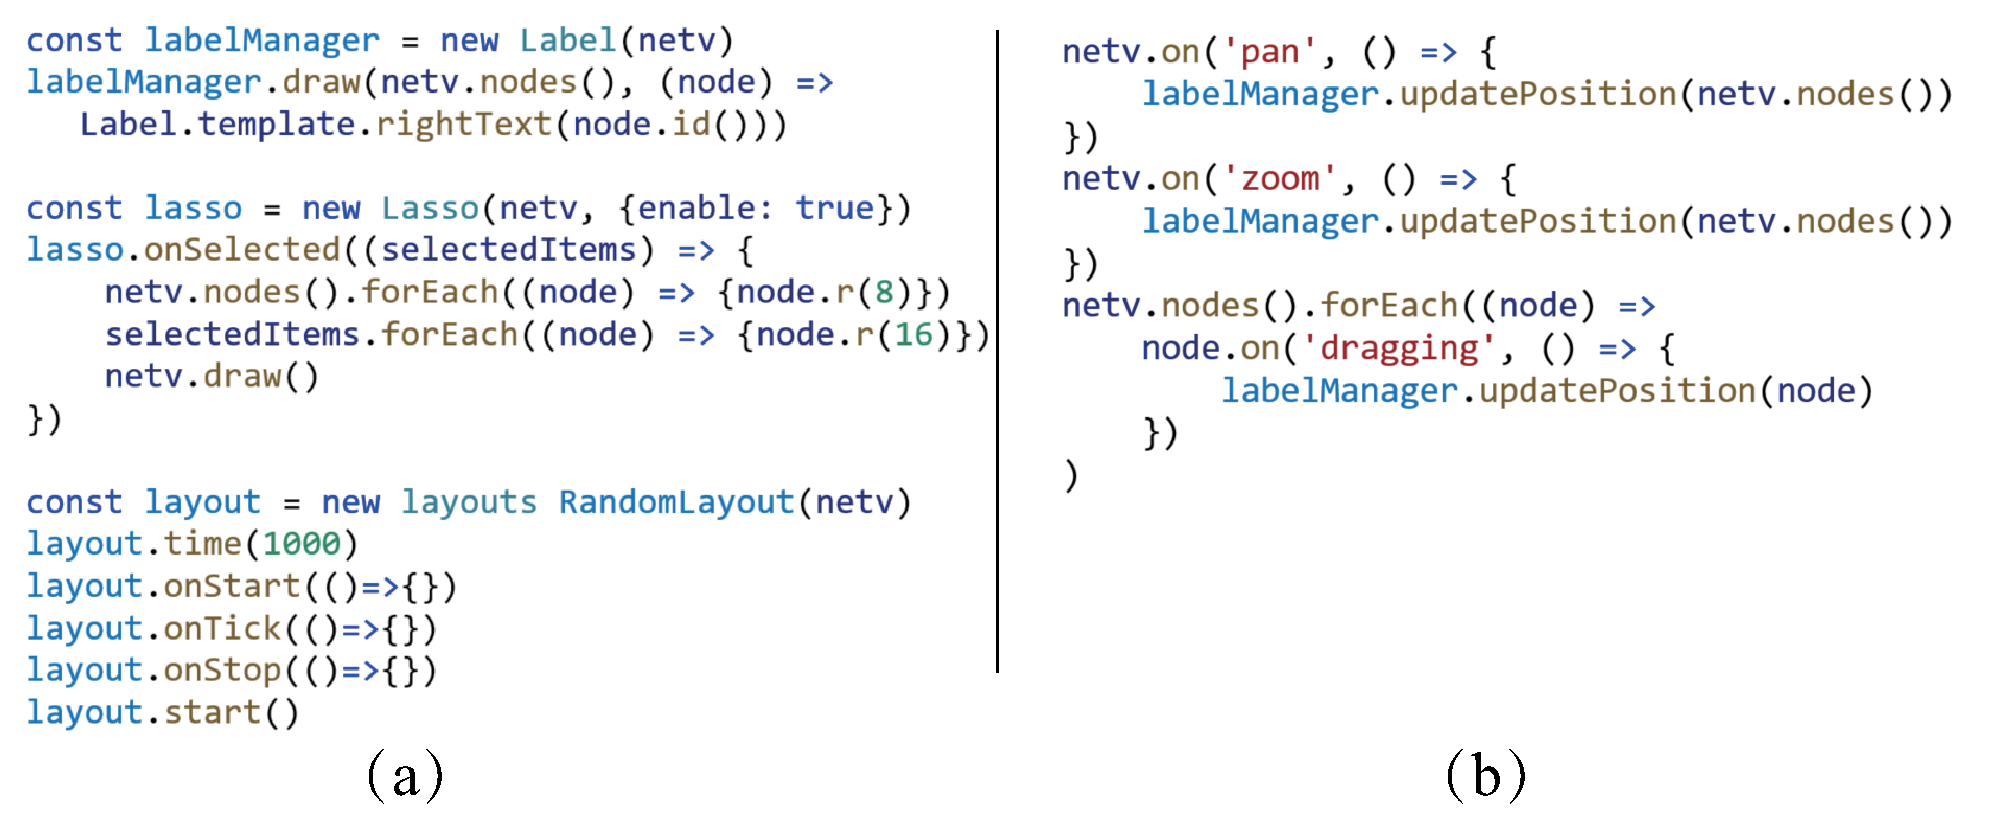
\includegraphics[width=\linewidth]{fig/ex8.eps}
    \caption{
        Code examples of (a) plugin configurations, and (b) build-in interactions.
    }
    \label{fig:ex8}
\end{figure}

% \subsection{Layout}
% \name supports various graph layout algorithms. Moreover, developers can implement by combining with external layouts such as D3.js (\autoref{fig:ex4} (a)), or by using \name plugins (\autoref{fig:ex4} (b)). When combining with external layouts, \name acts as a renderer to draw graph by layout results.
% When using \name layout plugins, it supports developers to controllers of all layout stages. \autoref{fig:ex5} (b) (c) (d) show the graph visualization with force-directed layout.
% \begin{figure}
%     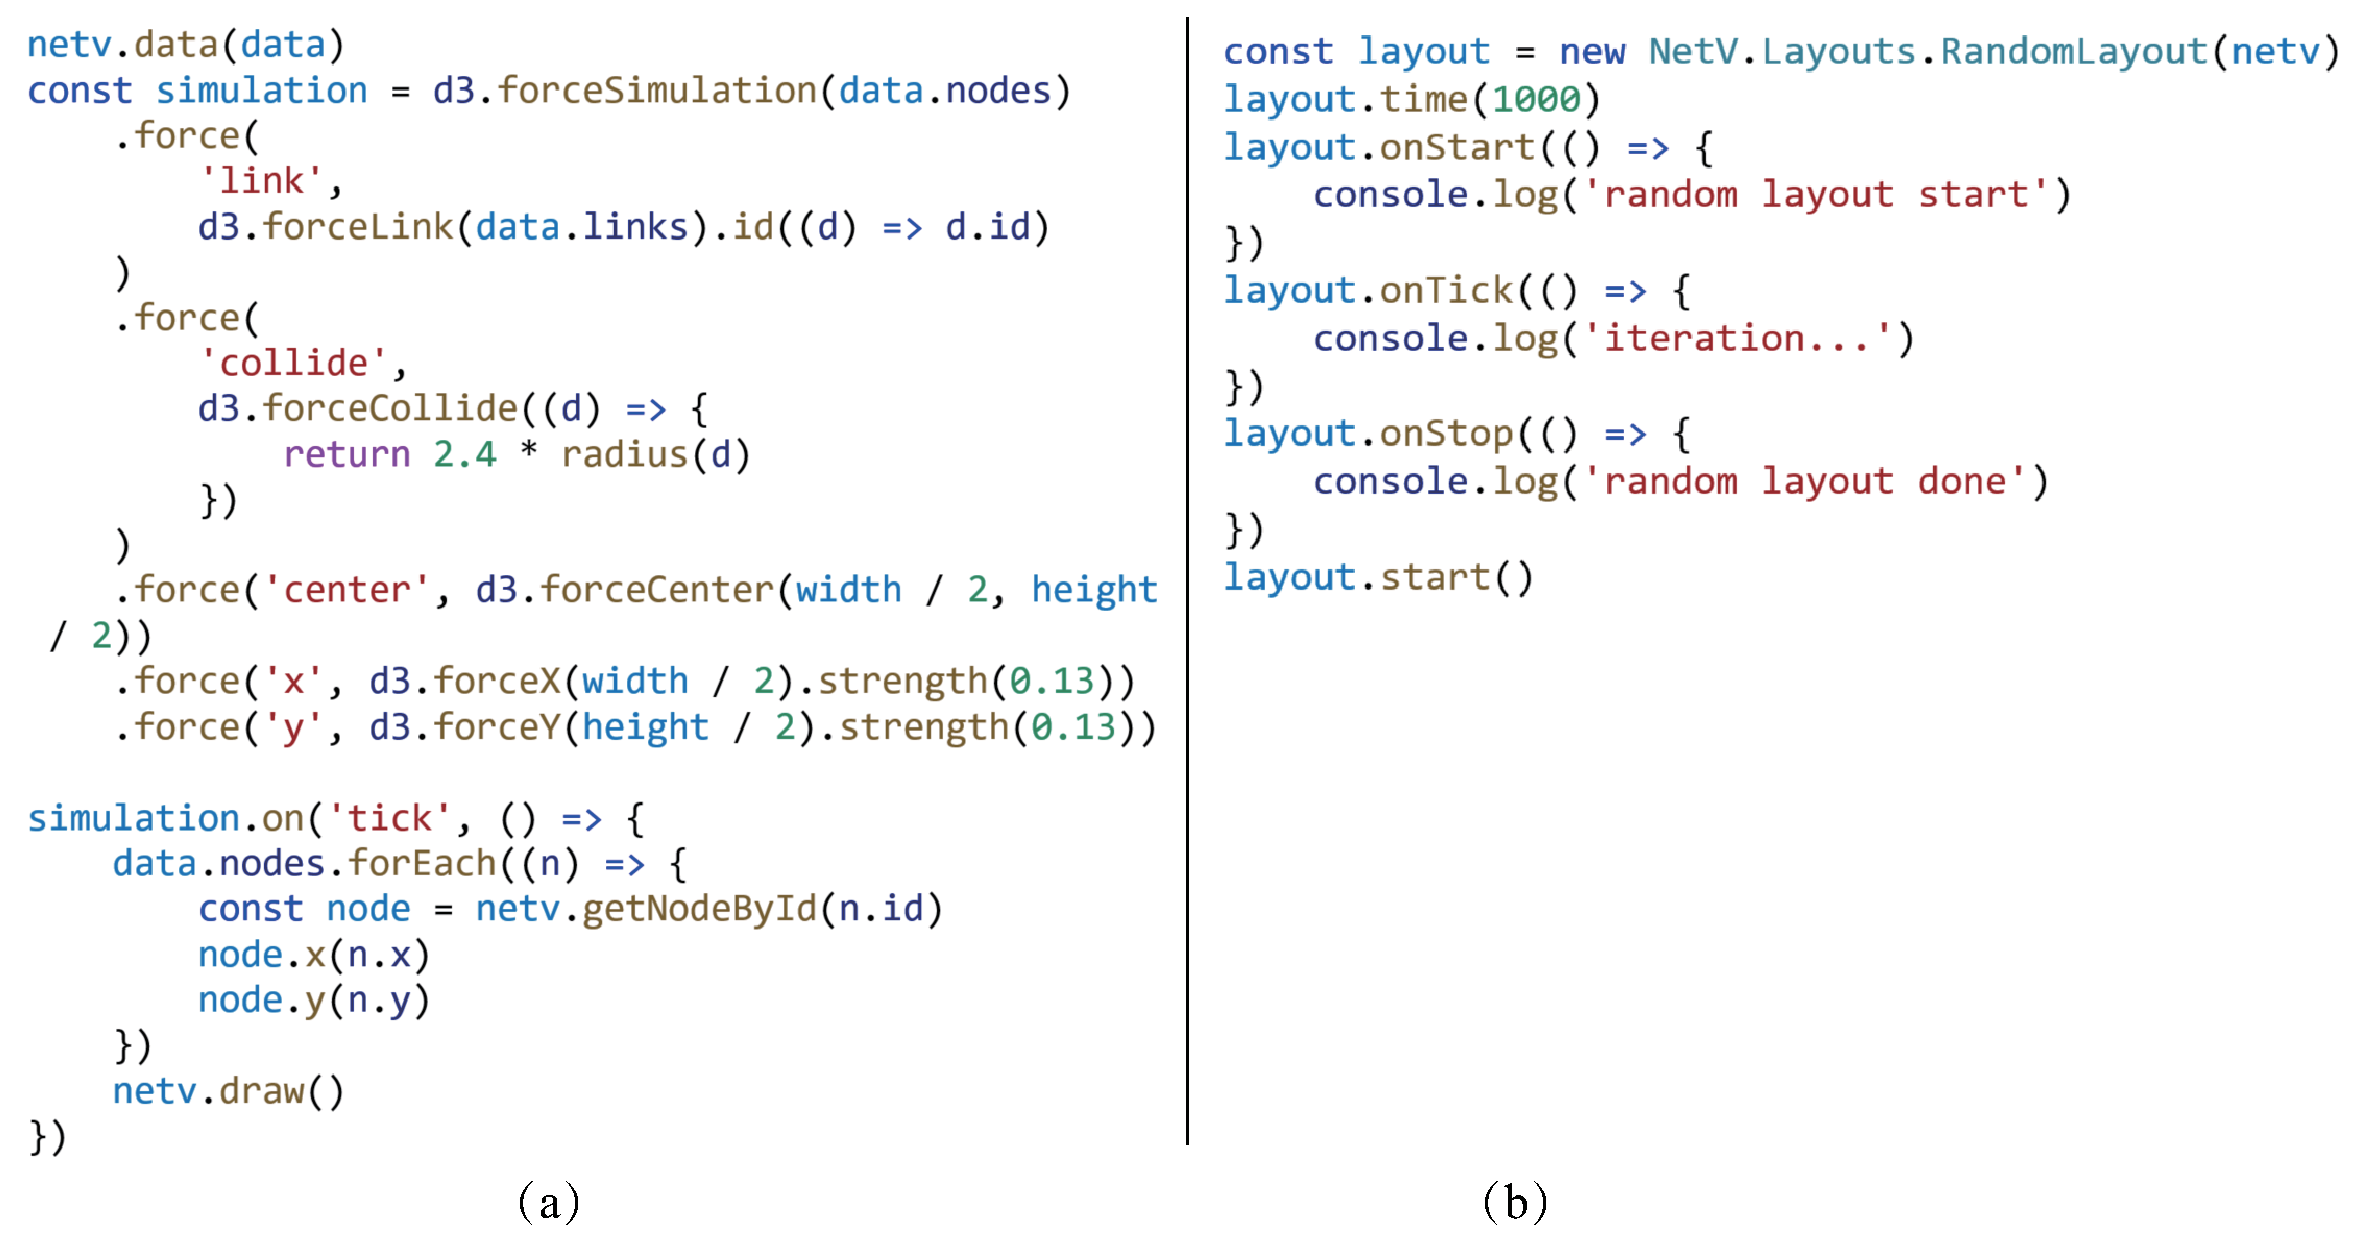
\includegraphics[width=\linewidth]{fig/ex4.eps}
%     \caption{
%         Layout. (a) Combining with D3.js. (b) Using \name plugins.
%     }
%     \label{fig:ex4}
% \end{figure}

\subsection{Large-Scale Graph}
\name aims to render large-scale graphs. \autoref{fig:ex5}(d) shows the graph visualization results of Finan512 dataset~\cite{davis2011university} with 74,752 nodes and 261,129 edges. \autoref{fig:ex5}(e) shows the graph visualization results of bcsstk31 dataset~\cite{davis2011university} with 35,590 nodes and 572,915 edges,  Thanks to WebGL, NetV.js can easily support rendering millions of elements.




% \begin{figure}
%     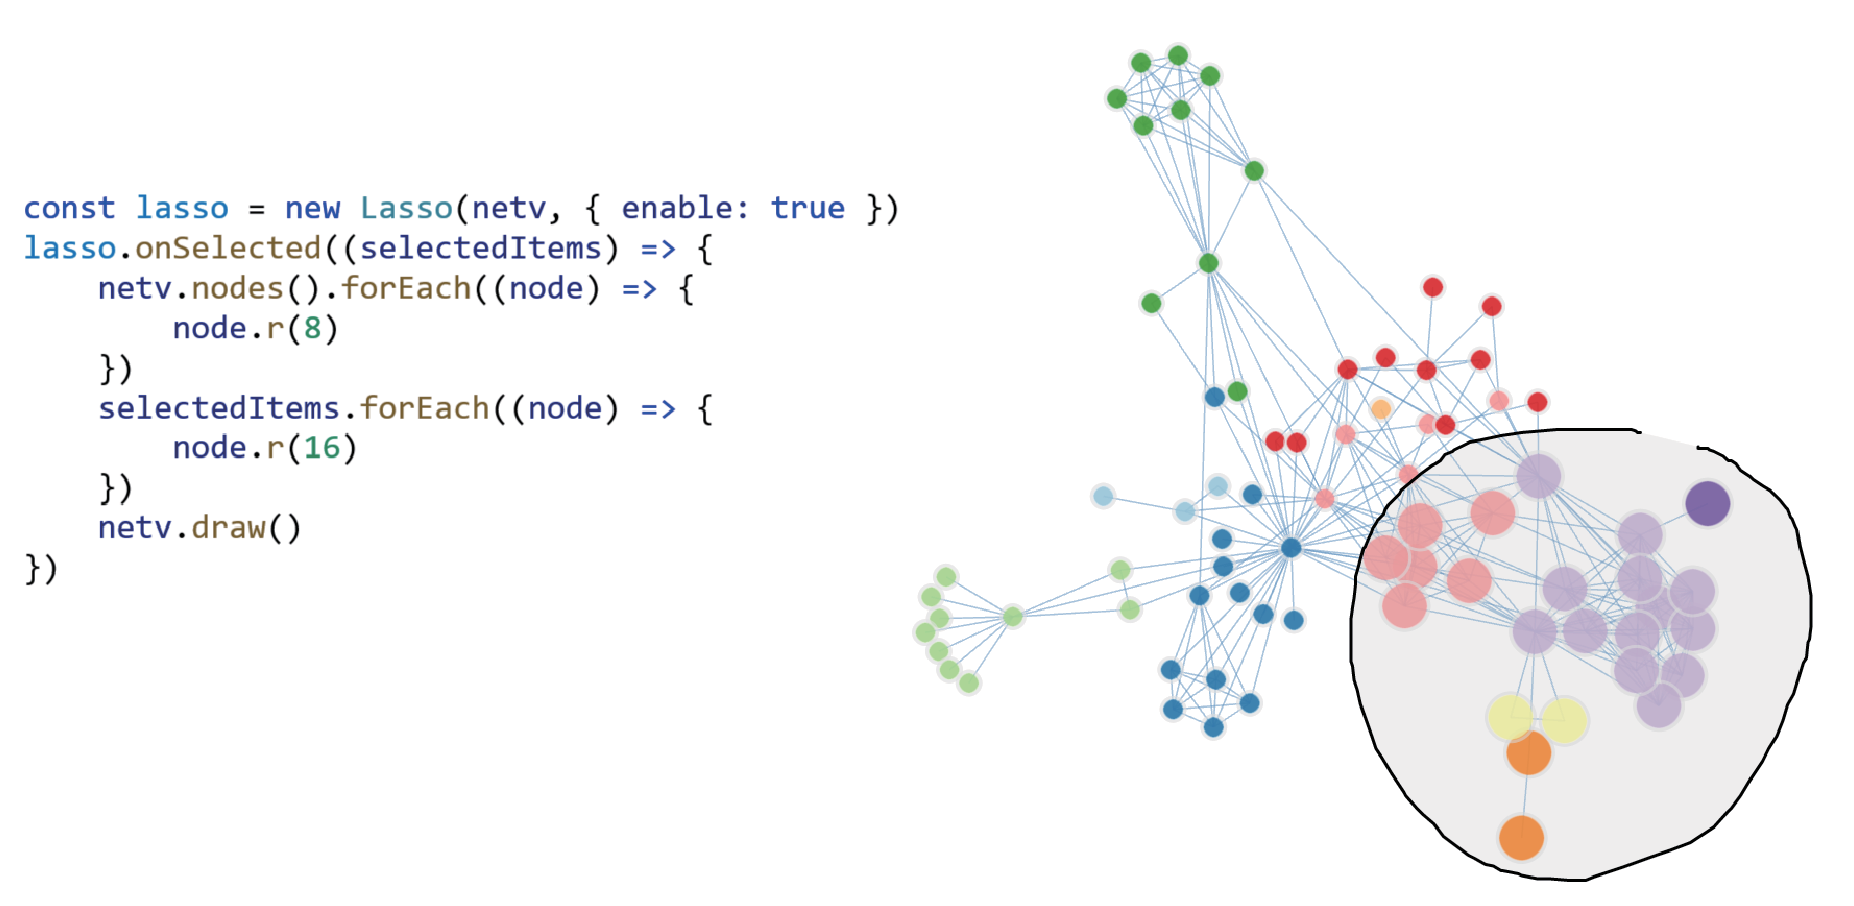
\includegraphics[width=\linewidth]{fig/ex7.eps}
%     \caption{
%         Label.
%     }
%     \label{fig:ex7}
% \end{figure}